\documentclass{article}
\usepackage{graphicx} % Required for inserting images
%Welcome :)

\documentclass{article}

% Basic document formatting
\usepackage[utf8]{inputenc}     % Input encoding
\usepackage[T1]{fontenc}        % Font encoding
\usepackage{lmodern}            % Modern LaTeX fonts
\usepackage{geometry}           % Set page margins
\geometry{a4paper, total={170mm,257mm}, left=20mm, top=20mm} 
\usepackage{float}              % Handling of floating elements
\usepackage{fancyhdr}           % Fancy headers
\usepackage{lastpage}           % use \pageref{LastPage} to make page x of y footers
\setlength{\parindent}{0pt}     % No \noindent

% Figures
\usepackage{graphicx}           % For including images
\usepackage{caption}            % Using the caption package
\usepackage{wrapfig}            % For including Wrap Figures
\usepackage{subcaption}         % For subfigures within a figure environment
\usepackage{pgfplots}           % Drawing plots
\usepackage{pgf-pie}            % For creating pie charts
\captionsetup[figure]{labelfont=bf}
\captionsetup[table]{labelfont=bf}
\usepackage{asymptote}          % Zum Zeichnen verschiedener Plots 
\usepackage{pdfpages}           % Zum Einfügen ganzer PDFs

% Colorboxes
\usepackage[skins]{tcolorbox}   % Color Boxes

% Tables and long tables
\usepackage{tabularx}           % Advanced table features
\usepackage{longtable}          % For tables that span multiple pages
\usepackage{multirow}           % Allows for multirow cells in tables
\usepackage{booktabs}           % For professional-quality tables

% Math packages
\usepackage{amsmath}            % Enhanced mathematical formatting
\usepackage{amssymb}            % Extended symbol collection
\usepackage{amsfonts}           % Mathematical fonts
\usepackage[version=4]{mhchem}  % Chemische Formeln
\usepackage{mathtools}          % Mathematical tools to supplement amsmath
\numberwithin{equation}{section} % Numbers Equations with chapters
\usepackage{siunitx}            % Makes SI-Units

% Code display
\usepackage{listings}           % For displaying code
\usepackage{xcolor}             % For coloring code
\lstdefinestyle{mystyle}{
    backgroundcolor=\color{backcolour},   
    commentstyle=\color{codegreen},
    keywordstyle=\color{ao},
    numberstyle=\tiny\color{codegray},
    basicstyle=\ttfamily\footnotesize,
    breakatwhitespace=false,         
    breaklines=true,                 
    captionpos=b,                    
    keepspaces=true,                 
    numbers=left,                    
    numbersep=5pt,                  
    showspaces=false,                
    showstringspaces=false,
    showtabs=false,                  
    tabsize=2
}
\lstset{style=mystyle}

% Custom Colours
\definecolor{LightCyan}{rgb}{0.88,1,1}
\definecolor{dkgreen}{rgb}{0,0.6,0}
\definecolor{gray}{rgb}{0.5,0.5,0.5}
\definecolor{mauve}{rgb}{0.58,0,0.82}
\definecolor{codegreen}{rgb}{0,0.6,0}
\definecolor{codegray}{rgb}{0.5,0.5,0.5}
\definecolor{ao}{rgb}{0.0, 0.0, 1.0}
\definecolor{backcolour}{rgb}{0.95,0.95,0.92}

% Referencing
\usepackage[style=numeric, backend=biber, sorting=none]{biblatex} % Imports biblatex package
\addbibresource{MAIN.bib} %Import the bibliography file
\DeclareFieldFormat{labelnumberwidth}{\mkbibbrackets{#1}} %ensure that the label numbers in the bibliography are enclosed in brackets.
\usepackage{xurl}

% Hyperlinks in the document
\usepackage{hyperref}           % For adding hyperlinks


\begin{document}

\vspace{-4cm}

\includegraphics[width=0.25\linewidth]{Graphics/VCS-Logo.png}

\vspace{-1.5cm}
\begin{flushright}
\parbox[r]{5cm}{Zurich, \today}
\end{flushright}

\vspace{1.5cm}
\begin{center}
\textbf{\LARGE{Vorschläge und Ideen der VCS zu PAKETH}} \\
\vspace{0.5cm}
\Large
VCS - Vereinigung der Studierenden der Chemie-, Biochemie – Chemische Biologie, 
Chemieingenieurwissenschaften und interdisziplinären Naturwissenschaften
\end{center}

\section{Lernzeit}
Die VCS bevorzugt stark eine Lernzeit von \textbf{4 Wochen}.

\section{Abmeldefrist von Prüfungen}
Wir glauben, dass eine möglichst späte Abmeldung von den Prüfungen unseren Studierenden eine wichtige Freiheit erlaubt. Bereits am Anfang des Semesters entscheiden zu müssen, welche Prüfungen man einige Monate später ablegen wird, ist eine große Herausforderung. Viele Studierende brauchen mehr als drei Wochen, um abschätzen zu können, ob sie die Prüfungen während der Prüfungssession ablegen möchten. Besonders im dritten Jahr Chemieingenieurwissenschaften ist aufgefallen, dass von zwei Blöcken des Herbstsemesters viele Studierende einen schieben. \\

Wir sehen einen großen Vorteil darin, die Abmeldung von einer Lerneinheit (und ihrer Prüfung) soweit wie möglich nach hinten zu verschieben, da es Studierende ermutigt, auch schwierige Fächer/Blöcke zu belegen. Es ist durchaus denkbar, dass sich weniger Studierende das zutrauen, wenn die Möglichkeit der Abmeldung der Prüfungen wegfällt. 

\section{Repetitionsphase}
Wir stimmen dem Vorschlag zu, die Repetitionsprüfungen vor den regulären Prüfungen anzubieten. Es erlaubt Studierenden, sich zuerst auf die Repetitionsprüfungen vorzubereiten.

\section{Orientierungssemester}
Wir möchten in der Diskussion um das Orientierungssemester gerne einbringen, dass wir dieses als sehr wichtig für Studierende empfinden. Das Orientierungssemester ist gedacht für Studierende, die zweimal einen Prüfungsblock nicht bestanden haben und somit aus dem Studienfach ausgeschlossen sind. Das Orientierungssemester bietet Studierenden die Möglichkeit, ein Semester nach dem Nicht-Bestehen weiter zu studieren und Fächer zu belegen, die außerhalb ihres vorherigen Fachgebiets liegen. Dies dient der Orientierung und bietet die Chance, Studierende nicht direkt aus dem Universitätskontext auszuschließen.\\

In Anbetracht der Tatsache, dass die Prüfungsergebnisse erst einige Tage vor Beginn des neuen Semesters veröffentlicht werden, ist es uns kaum ersichtlich, wie zu erwarten ist, dass eine Person sich so schnell auf einen neuen Studiengang/kein Studium entscheiden kann.\\

Uns ist wichtig, dass das Orientierungssemester weiterhin eine Möglichkeit bleibt, zumindest für die Studierenden, die nach dem zweiten oder dritten Jahr aus dem Studiengang ausgeschlossen werden, da sie der Ausschluss vom Studiengang besonders trifft.

\newpage
\section{Stundenplanvorschlag 1. Jahr}
Unsere Vorgänger haben die Initiative gestartet, einen überarbeiteten Stundenplanvorschlag auszuarbeiten. Wir haben es mit Studierenden diskutiert und sehen durch eine Aufteilung in zwei Gruppen einige Vorteile. Die Vorlesungen werden am Vormittag angeboten und die Laborzeiten aufgeteilt auf Montag, Dienstag, Mittwoch und Donnerstag Nachmittag. Das erlaubt die Unterbringung von mehr Studierenden im Praktikum während des Semesters, was in PAKETH-Zeiten erstrebenswert ist.

\begin{center}
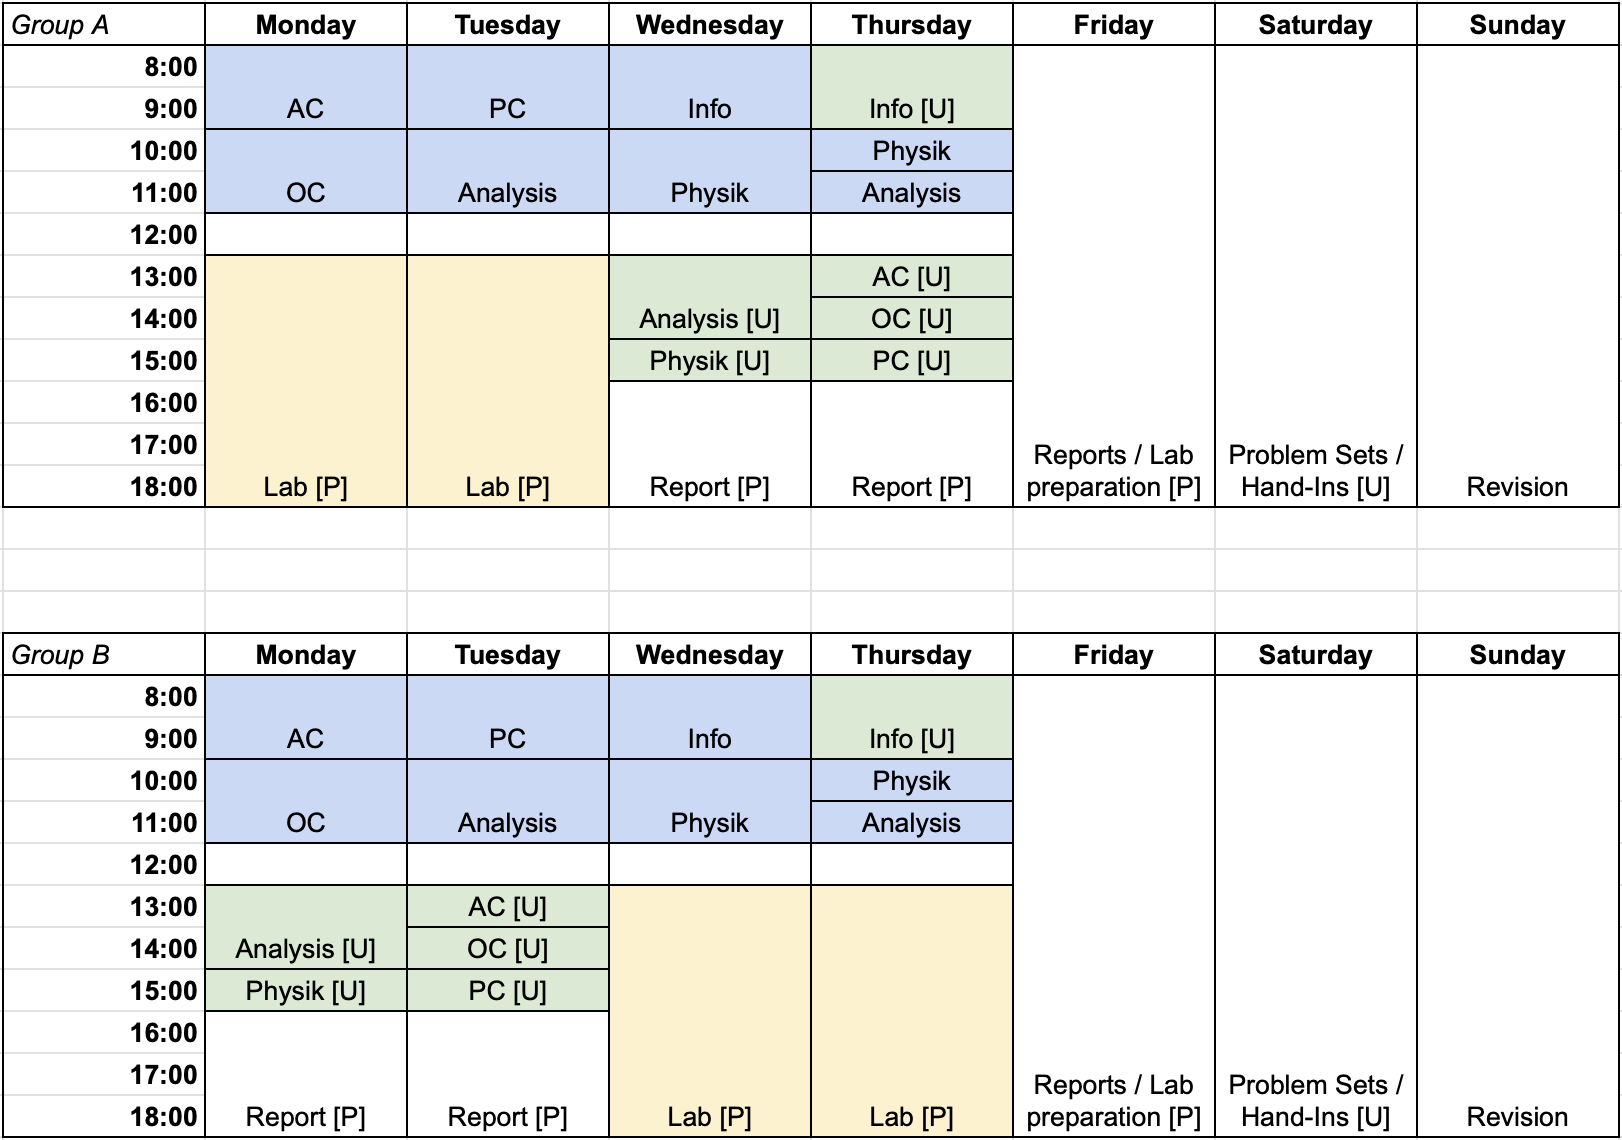
\includegraphics[width=0.9\linewidth]{Graphics/Screenshot 2024-11-08 at 07.54.10.png}
\end{center}

\end{document}
